\header{
    \headtitle{Au bal de l'Hôtel-Dieu} \label{au-bal-de-l-hotel-dieu}
    %
    
    \insertComment{Publiée en 1911 dans l'Antologie hospitalière et latinesque.}{L'Hôtel-Dieu est un refuge pour infirmes créé en 651 par l'\'Evèque Saint Landry}
}

\enluminure{4}{\href{https://www.youtube.com/watch?v=0gQyMM5g-ug}{A}}\\
$\left.\begin{tabular}{l}
\hspace{-0.4cm}
\textsc{u bal}  de l'Hôtel-Dieu, nom de Dieu ! ~~~~~~
\\
\hspace{-0.4cm}
Y avait une surveillante  ~~~~~
\end{tabular}\right\rbrace$ bis
\\Qu'avait tant d'amoureux , nom de Dieu !
\\Qu'ell'ne savait l'quel prendre.
\\\\\textbf{Refrain :}
\bistriplespace{Ah, nom de Dieu !}
{Sacré nom de Dieu, quelle allure, nom de Dieu !}
{Sacré nom de Dieu, quelle allure !}
\bisdouble{Qu'avait tant d'amoureux, nom de Dieu ! }
{Qu'ell'ne savait l'quel prendre.}
Un jour l'intern'de gard', nom de Dieu !
\\En mariag'la demande 
\\
\bisdouble{Un jour l'intern'de gard', nom de Dieu ! }
{En mariag'la demande }
Le pèr'ne dit pas non, nom de Dieu !
\\La mère est consentante, 
\\
\bisdouble{Le pèr'ne dit pas non, nom de Dieu ! ~~}
{La mère est consentante,}
Malgré tous les envieux, nom de Dieu !
\\Ils coucheront ensemble 
\\
\bisdouble{Malgré tous les envieux, nom de Dieu !}
{Ils coucheront ensemble }
Dans un grand lit carré, nom de Dieu !
\\Tout garni de guirlandes 
\\
\bisdouble{Dans un grand lit carré, nom de Dieu !}
{Tout garni de guirlandes}
Aux quatre coins du lit, nom de Dieu !
\\Quatr'carabins qui bandent, 
\\
\bisdouble{Aux quatre coins du lit, nom de Dieu !}
{Quatr'carabins qui bandent,}
La belle est au milieu, nom de Dieu !
\\Elle écarte les jambes 
\\
\bisdouble{La belle est au milieu, nom de Dieu ! ~~~~~~}
{Elle écarte les jambes }
Les règl's lui sort'nt du con, nom de Dieu !
\\Encor'toutes fumantes 
\\
\bisdouble{Les règl's lui sort'nt du con, nom de Dieu !}
{Encor'toutes fumantes }
Vous tous qui m'écoutez, nom de Dieu !
\\Y passerez la langue 
\begin{figure}[h!]
\centering
   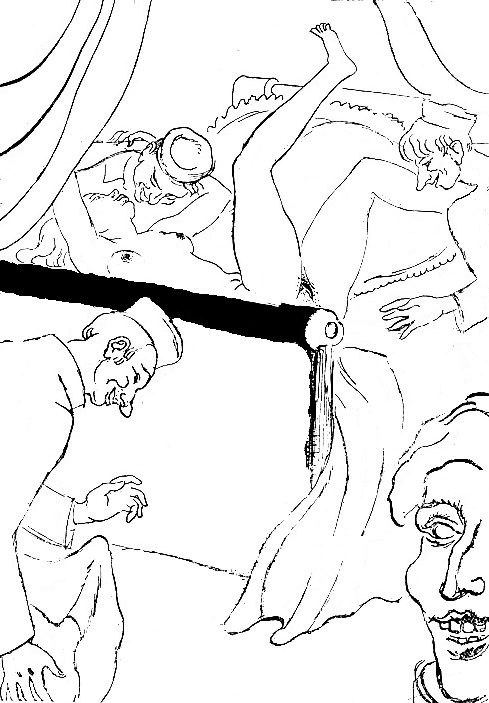
\includegraphics[width=0.6\textwidth]{images/ChansonHotelDieu.jpg}
 \end{figure}
\breakpage

